% Options for packages loaded elsewhere
\PassOptionsToPackage{unicode}{hyperref}
\PassOptionsToPackage{hyphens}{url}
%
\documentclass[
]{article}
\usepackage{amsmath,amssymb}
\usepackage{iftex}
\ifPDFTeX
  \usepackage[T1]{fontenc}
  \usepackage[utf8]{inputenc}
  \usepackage{textcomp} % provide euro and other symbols
\else % if luatex or xetex
  \usepackage{unicode-math} % this also loads fontspec
  \defaultfontfeatures{Scale=MatchLowercase}
  \defaultfontfeatures[\rmfamily]{Ligatures=TeX,Scale=1}
\fi
\usepackage{lmodern}
\ifPDFTeX\else
  % xetex/luatex font selection
\fi
% Use upquote if available, for straight quotes in verbatim environments
\IfFileExists{upquote.sty}{\usepackage{upquote}}{}
\IfFileExists{microtype.sty}{% use microtype if available
  \usepackage[]{microtype}
  \UseMicrotypeSet[protrusion]{basicmath} % disable protrusion for tt fonts
}{}
\makeatletter
\@ifundefined{KOMAClassName}{% if non-KOMA class
  \IfFileExists{parskip.sty}{%
    \usepackage{parskip}
  }{% else
    \setlength{\parindent}{0pt}
    \setlength{\parskip}{6pt plus 2pt minus 1pt}}
}{% if KOMA class
  \KOMAoptions{parskip=half}}
\makeatother
\usepackage{xcolor}
\usepackage[margin=1in]{geometry}
\usepackage{color}
\usepackage{fancyvrb}
\newcommand{\VerbBar}{|}
\newcommand{\VERB}{\Verb[commandchars=\\\{\}]}
\DefineVerbatimEnvironment{Highlighting}{Verbatim}{commandchars=\\\{\}}
% Add ',fontsize=\small' for more characters per line
\usepackage{framed}
\definecolor{shadecolor}{RGB}{248,248,248}
\newenvironment{Shaded}{\begin{snugshade}}{\end{snugshade}}
\newcommand{\AlertTok}[1]{\textcolor[rgb]{0.94,0.16,0.16}{#1}}
\newcommand{\AnnotationTok}[1]{\textcolor[rgb]{0.56,0.35,0.01}{\textbf{\textit{#1}}}}
\newcommand{\AttributeTok}[1]{\textcolor[rgb]{0.13,0.29,0.53}{#1}}
\newcommand{\BaseNTok}[1]{\textcolor[rgb]{0.00,0.00,0.81}{#1}}
\newcommand{\BuiltInTok}[1]{#1}
\newcommand{\CharTok}[1]{\textcolor[rgb]{0.31,0.60,0.02}{#1}}
\newcommand{\CommentTok}[1]{\textcolor[rgb]{0.56,0.35,0.01}{\textit{#1}}}
\newcommand{\CommentVarTok}[1]{\textcolor[rgb]{0.56,0.35,0.01}{\textbf{\textit{#1}}}}
\newcommand{\ConstantTok}[1]{\textcolor[rgb]{0.56,0.35,0.01}{#1}}
\newcommand{\ControlFlowTok}[1]{\textcolor[rgb]{0.13,0.29,0.53}{\textbf{#1}}}
\newcommand{\DataTypeTok}[1]{\textcolor[rgb]{0.13,0.29,0.53}{#1}}
\newcommand{\DecValTok}[1]{\textcolor[rgb]{0.00,0.00,0.81}{#1}}
\newcommand{\DocumentationTok}[1]{\textcolor[rgb]{0.56,0.35,0.01}{\textbf{\textit{#1}}}}
\newcommand{\ErrorTok}[1]{\textcolor[rgb]{0.64,0.00,0.00}{\textbf{#1}}}
\newcommand{\ExtensionTok}[1]{#1}
\newcommand{\FloatTok}[1]{\textcolor[rgb]{0.00,0.00,0.81}{#1}}
\newcommand{\FunctionTok}[1]{\textcolor[rgb]{0.13,0.29,0.53}{\textbf{#1}}}
\newcommand{\ImportTok}[1]{#1}
\newcommand{\InformationTok}[1]{\textcolor[rgb]{0.56,0.35,0.01}{\textbf{\textit{#1}}}}
\newcommand{\KeywordTok}[1]{\textcolor[rgb]{0.13,0.29,0.53}{\textbf{#1}}}
\newcommand{\NormalTok}[1]{#1}
\newcommand{\OperatorTok}[1]{\textcolor[rgb]{0.81,0.36,0.00}{\textbf{#1}}}
\newcommand{\OtherTok}[1]{\textcolor[rgb]{0.56,0.35,0.01}{#1}}
\newcommand{\PreprocessorTok}[1]{\textcolor[rgb]{0.56,0.35,0.01}{\textit{#1}}}
\newcommand{\RegionMarkerTok}[1]{#1}
\newcommand{\SpecialCharTok}[1]{\textcolor[rgb]{0.81,0.36,0.00}{\textbf{#1}}}
\newcommand{\SpecialStringTok}[1]{\textcolor[rgb]{0.31,0.60,0.02}{#1}}
\newcommand{\StringTok}[1]{\textcolor[rgb]{0.31,0.60,0.02}{#1}}
\newcommand{\VariableTok}[1]{\textcolor[rgb]{0.00,0.00,0.00}{#1}}
\newcommand{\VerbatimStringTok}[1]{\textcolor[rgb]{0.31,0.60,0.02}{#1}}
\newcommand{\WarningTok}[1]{\textcolor[rgb]{0.56,0.35,0.01}{\textbf{\textit{#1}}}}
\usepackage{graphicx}
\makeatletter
\def\maxwidth{\ifdim\Gin@nat@width>\linewidth\linewidth\else\Gin@nat@width\fi}
\def\maxheight{\ifdim\Gin@nat@height>\textheight\textheight\else\Gin@nat@height\fi}
\makeatother
% Scale images if necessary, so that they will not overflow the page
% margins by default, and it is still possible to overwrite the defaults
% using explicit options in \includegraphics[width, height, ...]{}
\setkeys{Gin}{width=\maxwidth,height=\maxheight,keepaspectratio}
% Set default figure placement to htbp
\makeatletter
\def\fps@figure{htbp}
\makeatother
\setlength{\emergencystretch}{3em} % prevent overfull lines
\providecommand{\tightlist}{%
  \setlength{\itemsep}{0pt}\setlength{\parskip}{0pt}}
\setcounter{secnumdepth}{-\maxdimen} % remove section numbering
\usepackage{fancyhdr}
\usepackage{lipsum}
\pagestyle{fancy}
\fancyhead[R]{\thepage}
\fancypagestyle{plain}{\pagestyle{fancy}}
\ifLuaTeX
  \usepackage{selnolig}  % disable illegal ligatures
\fi
\IfFileExists{bookmark.sty}{\usepackage{bookmark}}{\usepackage{hyperref}}
\IfFileExists{xurl.sty}{\usepackage{xurl}}{} % add URL line breaks if available
\urlstyle{same}
\hypersetup{
  pdftitle={Data Science II Homework 2},
  pdfauthor={Camille Okonkwo},
  hidelinks,
  pdfcreator={LaTeX via pandoc}}

\title{Data Science II Homework 2}
\author{Camille Okonkwo}
\date{}

\begin{document}
\maketitle

{
\setcounter{tocdepth}{2}
\tableofcontents
}
\newpage

\begin{Shaded}
\begin{Highlighting}[]
\FunctionTok{library}\NormalTok{(tidymodels)}
\FunctionTok{library}\NormalTok{(splines)}
\FunctionTok{library}\NormalTok{(earth)}
\end{Highlighting}
\end{Shaded}

Partition the dataset into two parts: training data (80\%) and test data
(20\%) with \texttt{tidymodels}.

\begin{Shaded}
\begin{Highlighting}[]
\NormalTok{college }\OtherTok{=} \FunctionTok{read\_csv}\NormalTok{(}\StringTok{"data/College.csv"}\NormalTok{) }\SpecialCharTok{|\textgreater{}}
  \FunctionTok{drop\_na}\NormalTok{() }\SpecialCharTok{|\textgreater{}} 
  \FunctionTok{select}\NormalTok{(}\SpecialCharTok{{-}}\NormalTok{College)}
\end{Highlighting}
\end{Shaded}

\begin{verbatim}
## Rows: 565 Columns: 18
## -- Column specification --------------------------------------------------------
## Delimiter: ","
## chr  (1): College
## dbl (17): Apps, Accept, Enroll, Top10perc, Top25perc, F.Undergrad, P.Undergr...
## 
## i Use `spec()` to retrieve the full column specification for this data.
## i Specify the column types or set `show_col_types = FALSE` to quiet this message.
\end{verbatim}

\begin{Shaded}
\begin{Highlighting}[]
\FunctionTok{set.seed}\NormalTok{(}\DecValTok{2}\NormalTok{)}

\CommentTok{\# create a random split of 80\% training and 20\% test data}
\NormalTok{data\_split }\OtherTok{\textless{}{-}} \FunctionTok{initial\_split}\NormalTok{(}\AttributeTok{data =}\NormalTok{ college, }\AttributeTok{prop =} \FloatTok{0.8}\NormalTok{)}

\CommentTok{\# partitioned datasets}
\NormalTok{training\_data }\OtherTok{=} \FunctionTok{training}\NormalTok{(data\_split)}

\NormalTok{testing\_data }\OtherTok{=} \FunctionTok{testing}\NormalTok{(data\_split)}

\FunctionTok{head}\NormalTok{(training\_data)}
\end{Highlighting}
\end{Shaded}

\begin{verbatim}
## # A tibble: 6 x 17
##    Apps Accept Enroll Top10perc Top25perc F.Undergrad P.Undergrad Outstate
##   <dbl>  <dbl>  <dbl>     <dbl>     <dbl>       <dbl>       <dbl>    <dbl>
## 1  1380    768    263        57        82        1000         105    19300
## 2   434    321    141        28        53         624         269    10950
## 3  2013   1053    212        33        61         912         158     5150
## 4  2324   1319    370        52        81        1686          35    16560
## 5  1709   1385    634        36        72        2281          50    14125
## 6   427    385    143        18        38         581         533    12700
## # i 9 more variables: Room.Board <dbl>, Books <dbl>, Personal <dbl>, PhD <dbl>,
## #   Terminal <dbl>, S.F.Ratio <dbl>, perc.alumni <dbl>, Expend <dbl>,
## #   Grad.Rate <dbl>
\end{verbatim}

\begin{Shaded}
\begin{Highlighting}[]
\FunctionTok{head}\NormalTok{(testing\_data)}
\end{Highlighting}
\end{Shaded}

\begin{verbatim}
## # A tibble: 6 x 17
##    Apps Accept Enroll Top10perc Top25perc F.Undergrad P.Undergrad Outstate
##   <dbl>  <dbl>  <dbl>     <dbl>     <dbl>       <dbl>       <dbl>    <dbl>
## 1  2186   1924    512        16        29        2683        1227    12280
## 2  1428   1097    336        22        50        1036          99    11250
## 3   193    146     55        16        44         249         869     7560
## 4   582    498    172        21        44         799          78    10468
## 5  1732   1425    472        37        75        1830         110    16548
## 6   494    313    157        23        46        1317        1235     8352
## # i 9 more variables: Room.Board <dbl>, Books <dbl>, Personal <dbl>, PhD <dbl>,
## #   Terminal <dbl>, S.F.Ratio <dbl>, perc.alumni <dbl>, Expend <dbl>,
## #   Grad.Rate <dbl>
\end{verbatim}

\begin{Shaded}
\begin{Highlighting}[]
\CommentTok{\# creating a matrix of predictors and vector of response for each data set}

\CommentTok{\# training data}
\NormalTok{x }\OtherTok{\textless{}{-}} \FunctionTok{model.matrix}\NormalTok{(Outstate }\SpecialCharTok{\textasciitilde{}}\NormalTok{ ., training\_data)[, }\SpecialCharTok{{-}}\DecValTok{1}\NormalTok{] }\CommentTok{\# matrix of predictors}
\FunctionTok{head}\NormalTok{(x)}
\end{Highlighting}
\end{Shaded}

\begin{verbatim}
##   Apps Accept Enroll Top10perc Top25perc F.Undergrad P.Undergrad Room.Board
## 1 1380    768    263        57        82        1000         105       6694
## 2  434    321    141        28        53         624         269       4600
## 3 2013   1053    212        33        61         912         158       3036
## 4 2324   1319    370        52        81        1686          35       5140
## 5 1709   1385    634        36        72        2281          50       3600
## 6  427    385    143        18        38         581         533       5800
##   Books Personal PhD Terminal S.F.Ratio perc.alumni Expend Grad.Rate
## 1   600      700  89       93       6.1          18  14779        83
## 2   550      950  79       82      12.9          30   9264        81
## 3   500     1655  64       74      10.5          11   7547        59
## 4   558     1152  91       93      10.5          30  16196        79
## 5   400      700  79       89      12.5          58   9907        80
## 6   450      700  81       85      10.3          37  11758        84
\end{verbatim}

\begin{Shaded}
\begin{Highlighting}[]
\NormalTok{y }\OtherTok{\textless{}{-}}\NormalTok{ training\_data}\SpecialCharTok{$}\NormalTok{Outstate }\CommentTok{\# vector of response}

\CommentTok{\# testing data}
\NormalTok{x2 }\OtherTok{\textless{}{-}} \FunctionTok{model.matrix}\NormalTok{(Outstate }\SpecialCharTok{\textasciitilde{}}\NormalTok{ .,testing\_data)[, }\SpecialCharTok{{-}}\DecValTok{1}\NormalTok{] }\CommentTok{\# matrix of predictors}
\NormalTok{y2 }\OtherTok{\textless{}{-}}\NormalTok{ testing\_data}\SpecialCharTok{$}\NormalTok{Outstate }\CommentTok{\# vector of response}
\end{Highlighting}
\end{Shaded}

\hypertarget{a-fit-smoothing-spline-models-to-predict-out-of-state-tuition-outstate-using-the-percentage-of-alumni-who-donate-perc.alumni-as-the-only-predictor-across-a-range-of-degrees-of-freedom.-plot-the-model-fits-for-each-degree-of-freedom.-describe-the-observed-patterns-that-emerge-with-varying-degrees-of-freedom.-select-an-appropriate-degree-of-freedom-for-the-model-and-plot-this-optimal-fit.-explain-the-criteria-you-used-to-determine-the-best-choice-of-degree-of-freedom.}{%
\section{1a) Fit smoothing spline models to predict out-of-state tuition
(Outstate) using the percentage of alumni who donate (perc.alumni) as
the only predictor, across a range of degrees of freedom. Plot the model
fits for each degree of freedom. Describe the observed patterns that
emerge with varying degrees of freedom. Select an appropriate degree of
freedom for the model and plot this optimal fit. Explain the criteria
you used to determine the best choice of degree of
freedom.}\label{a-fit-smoothing-spline-models-to-predict-out-of-state-tuition-outstate-using-the-percentage-of-alumni-who-donate-perc.alumni-as-the-only-predictor-across-a-range-of-degrees-of-freedom.-plot-the-model-fits-for-each-degree-of-freedom.-describe-the-observed-patterns-that-emerge-with-varying-degrees-of-freedom.-select-an-appropriate-degree-of-freedom-for-the-model-and-plot-this-optimal-fit.-explain-the-criteria-you-used-to-determine-the-best-choice-of-degree-of-freedom.}}

\begin{Shaded}
\begin{Highlighting}[]
\FunctionTok{library}\NormalTok{(splines)}

\CommentTok{\# create a grid for x}
\NormalTok{perc.alumni.grid }\OtherTok{\textless{}{-}} \FunctionTok{seq}\NormalTok{(}\DecValTok{0}\NormalTok{, }\FunctionTok{max}\NormalTok{(college}\SpecialCharTok{$}\NormalTok{perc.alumni) }\SpecialCharTok{+} \DecValTok{5}\NormalTok{, }\AttributeTok{by =} \DecValTok{1}\NormalTok{)}

\CommentTok{\# loop prep}
\NormalTok{fit.ss }\OtherTok{=} \FunctionTok{list}\NormalTok{()}
\NormalTok{pred.ss }\OtherTok{=} \FunctionTok{list}\NormalTok{()}
\NormalTok{pred.ss.df }\OtherTok{=} \FunctionTok{list}\NormalTok{()}
\NormalTok{pred.ss.df.range }\OtherTok{=} \FunctionTok{data.frame}\NormalTok{()}

\FunctionTok{set.seed}\NormalTok{(}\DecValTok{2}\NormalTok{)}
\CommentTok{\# loop for a range of degrees of freedom}
\ControlFlowTok{for}\NormalTok{ (i }\ControlFlowTok{in} \FloatTok{1.1}\SpecialCharTok{:}\DecValTok{20}\NormalTok{) \{}
\NormalTok{  fit.ss[[i]] }\OtherTok{=} \FunctionTok{smooth.spline}\NormalTok{(training\_data}\SpecialCharTok{$}\NormalTok{perc.alumni, training\_data}\SpecialCharTok{$}\NormalTok{Outstate, }\AttributeTok{df =}\NormalTok{ i)}
\NormalTok{  pred.ss[[i]] }\OtherTok{=} \FunctionTok{predict}\NormalTok{(fit.ss[[i]], }\AttributeTok{x =}\NormalTok{ perc.alumni.grid)}
\NormalTok{  pred.ss.df[[i]] }\OtherTok{=} \FunctionTok{data.frame}\NormalTok{(}\AttributeTok{pred =}\NormalTok{ pred.ss[[i]]}\SpecialCharTok{$}\NormalTok{y, }\AttributeTok{perc.alumni =}\NormalTok{ perc.alumni.grid, }\AttributeTok{df =}\NormalTok{ i)}
\NormalTok{  pred.ss.df.range }\OtherTok{=} \FunctionTok{rbind}\NormalTok{(pred.ss.df[[i]], pred.ss.df.range)}
\NormalTok{\}}

\CommentTok{\# scatter plot}
\NormalTok{p }\OtherTok{\textless{}{-}} \FunctionTok{ggplot}\NormalTok{(}\AttributeTok{data =}\NormalTok{ training\_data, }\FunctionTok{aes}\NormalTok{(}\AttributeTok{x =}\NormalTok{ perc.alumni, }\AttributeTok{y =}\NormalTok{ Outstate)) }\SpecialCharTok{+} \FunctionTok{geom\_point}\NormalTok{(}\AttributeTok{color =} \FunctionTok{rgb}\NormalTok{(}\FloatTok{0.2}\NormalTok{, }\FloatTok{0.4}\NormalTok{, }\FloatTok{0.2}\NormalTok{, }\FloatTok{0.5}\NormalTok{))}

\CommentTok{\# plot the model fits for each degree of freedom}
\NormalTok{p }\SpecialCharTok{+}
  \FunctionTok{geom\_line}\NormalTok{(}\FunctionTok{aes}\NormalTok{(}\AttributeTok{x =}\NormalTok{ perc.alumni, }\AttributeTok{y =}\NormalTok{ pred, }\AttributeTok{group =}\NormalTok{ df, }\AttributeTok{color =}\NormalTok{ df), }\AttributeTok{data =}\NormalTok{ pred.ss.df.range) }\SpecialCharTok{+} \FunctionTok{theme\_bw}\NormalTok{()}
\end{Highlighting}
\end{Shaded}

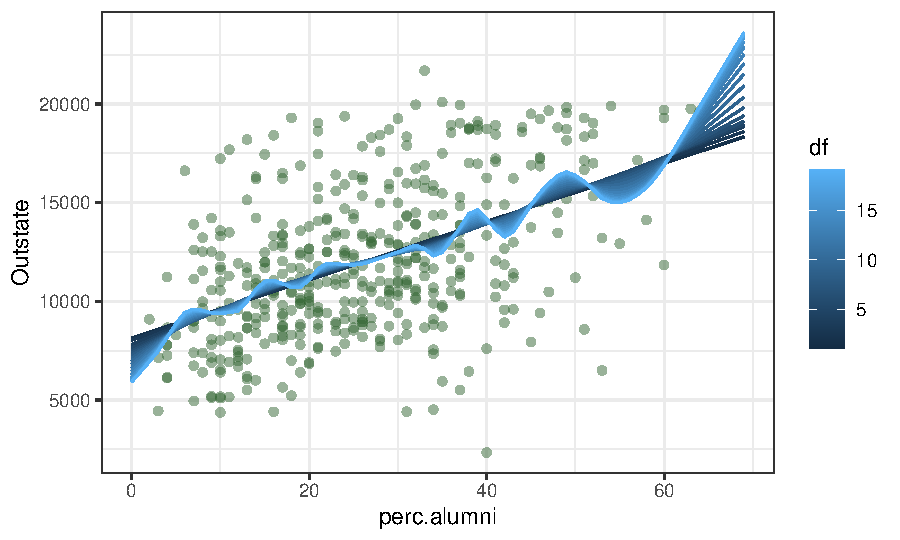
\includegraphics[width=0.9\linewidth]{HW2_co2554_files/figure-latex/smoothing_spline-1}

\begin{Shaded}
\begin{Highlighting}[]
\FunctionTok{set.seed}\NormalTok{(}\DecValTok{2}\NormalTok{)}

\CommentTok{\# select an appropriate degree of freedom for the model }
\NormalTok{fit.ss.optimal }\OtherTok{=} \FunctionTok{smooth.spline}\NormalTok{(training\_data}\SpecialCharTok{$}\NormalTok{perc.alumni, training\_data}\SpecialCharTok{$}\NormalTok{Outstate)}

\NormalTok{fit.ss.optimal}\SpecialCharTok{$}\NormalTok{df}
\end{Highlighting}
\end{Shaded}

\begin{verbatim}
## [1] 2.000245
\end{verbatim}

\begin{Shaded}
\begin{Highlighting}[]
\CommentTok{\# predicted values}
\NormalTok{pred.ss.optimal }\OtherTok{\textless{}{-}} \FunctionTok{predict}\NormalTok{(fit.ss.optimal,}
                   \AttributeTok{x =}\NormalTok{ perc.alumni.grid)}

\NormalTok{pred.ss.optimal.df }\OtherTok{\textless{}{-}} \FunctionTok{data.frame}\NormalTok{(}\AttributeTok{pred =}\NormalTok{ pred.ss.optimal}\SpecialCharTok{$}\NormalTok{y,}
                         \AttributeTok{perc.alumni =}\NormalTok{ perc.alumni.grid)}

\CommentTok{\# plot this optimal fit}
\NormalTok{p.optimal }\OtherTok{\textless{}{-}} \FunctionTok{ggplot}\NormalTok{(}\AttributeTok{data =}\NormalTok{ training\_data, }\FunctionTok{aes}\NormalTok{(}\AttributeTok{x =}\NormalTok{ perc.alumni, }\AttributeTok{y =}\NormalTok{ Outstate)) }\SpecialCharTok{+} \FunctionTok{geom\_point}\NormalTok{(}\AttributeTok{color =} \FunctionTok{rgb}\NormalTok{(}\FloatTok{0.2}\NormalTok{, }\FloatTok{0.4}\NormalTok{, }\FloatTok{0.2}\NormalTok{, }\FloatTok{0.5}\NormalTok{))}
  
\NormalTok{p.optimal }\SpecialCharTok{+}
  \FunctionTok{geom\_line}\NormalTok{(}\FunctionTok{aes}\NormalTok{(}\AttributeTok{x =}\NormalTok{ perc.alumni, }\AttributeTok{y =}\NormalTok{ pred), }\AttributeTok{data =}\NormalTok{ pred.ss.optimal.df,}
            \AttributeTok{color =} \FunctionTok{rgb}\NormalTok{(}\FloatTok{0.8}\NormalTok{, }\FloatTok{0.1}\NormalTok{, }\FloatTok{0.1}\NormalTok{, }\DecValTok{1}\NormalTok{)) }\SpecialCharTok{+} \FunctionTok{theme\_bw}\NormalTok{()}
\end{Highlighting}
\end{Shaded}

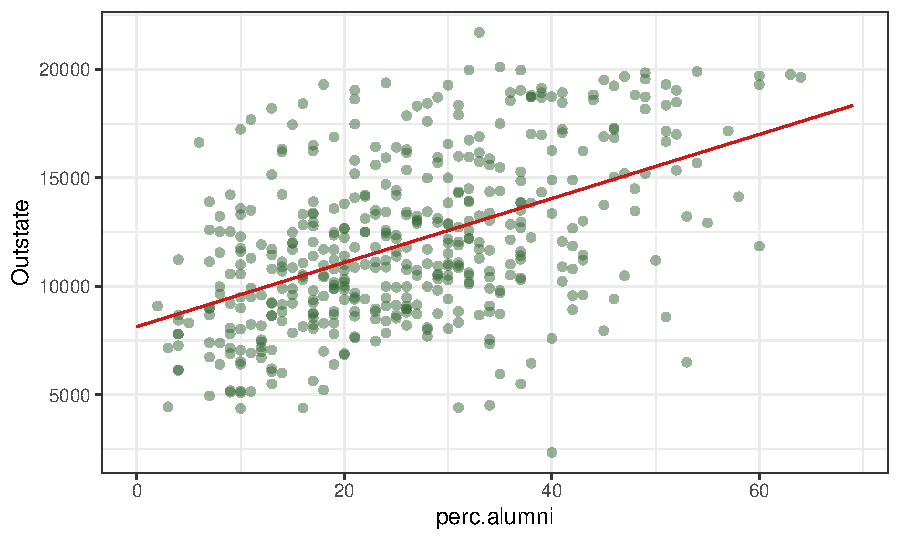
\includegraphics[width=0.9\linewidth]{HW2_co2554_files/figure-latex/smoothing_spline-2}
When the degrees of freedom is smaller, the model resembles a linear
model. As the degrees of freedom increase, the model becomes more
flexible and we can see that exemplified through the wavy lines. For the
optimal smoothing splines model, the degrees of freedom = 2.0002451. To
determine the best choice of degrees of freedom, we can use
cross-validation to choose the degrees of freedom that result in the
best predictive performance.

\newpage

\hypertarget{b-train-a-multivariate-adaptive-regression-spline-mars-model-to-predict-the-response-variable.-report-the-regression-function.-present-the-partial-dependence-plot-of-an-arbitrary-predictor-in-your-model.-report-the-test-error.}{%
\section{1b) Train a multivariate adaptive regression spline (MARS)
model to predict the response variable. Report the regression function.
Present the partial dependence plot of an arbitrary predictor in your
model. Report the test
error.}\label{b-train-a-multivariate-adaptive-regression-spline-mars-model-to-predict-the-response-variable.-report-the-regression-function.-present-the-partial-dependence-plot-of-an-arbitrary-predictor-in-your-model.-report-the-test-error.}}

\begin{Shaded}
\begin{Highlighting}[]
\FunctionTok{library}\NormalTok{(earth)}
\FunctionTok{library}\NormalTok{(caret)}
\end{Highlighting}
\end{Shaded}

\begin{verbatim}
## Loading required package: lattice
\end{verbatim}

\begin{verbatim}
## 
## Attaching package: 'caret'
\end{verbatim}

\begin{verbatim}
## The following objects are masked from 'package:yardstick':
## 
##     precision, recall, sensitivity, specificity
\end{verbatim}

\begin{verbatim}
## The following object is masked from 'package:purrr':
## 
##     lift
\end{verbatim}

\begin{Shaded}
\begin{Highlighting}[]
\CommentTok{\# 10{-}fold cross{-}validation}
\NormalTok{ctrl }\OtherTok{\textless{}{-}} \FunctionTok{trainControl}\NormalTok{(}\AttributeTok{method =} \StringTok{"cv"}\NormalTok{, }\AttributeTok{number =} \DecValTok{10}\NormalTok{)}

\CommentTok{\# set grid}
\NormalTok{mars\_grid }\OtherTok{\textless{}{-}} \FunctionTok{expand.grid}\NormalTok{(}\AttributeTok{degree =} \DecValTok{1}\SpecialCharTok{:}\DecValTok{3}\NormalTok{, }\AttributeTok{nprune =} \DecValTok{2}\SpecialCharTok{:}\DecValTok{15}\NormalTok{)}

\FunctionTok{set.seed}\NormalTok{(}\DecValTok{2}\NormalTok{)}

\CommentTok{\# fit a MARS model}
\NormalTok{mars.fit }\OtherTok{\textless{}{-}} \FunctionTok{train}\NormalTok{(x, y,}
                  \AttributeTok{method =} \StringTok{"earth"}\NormalTok{,}
                  \AttributeTok{tuneGrid =}\NormalTok{ mars\_grid,}
                  \AttributeTok{trControl =}\NormalTok{ ctrl)}
\CommentTok{\# plot}
\FunctionTok{ggplot}\NormalTok{(mars.fit)}
\end{Highlighting}
\end{Shaded}

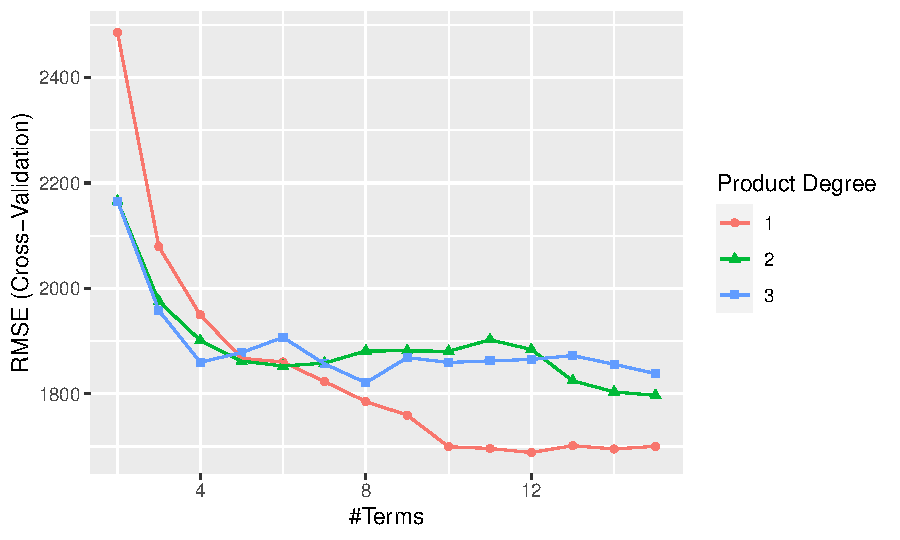
\includegraphics[width=0.9\linewidth]{HW2_co2554_files/figure-latex/MARS-1}

\begin{Shaded}
\begin{Highlighting}[]
\CommentTok{\# best tuning parameters}
\NormalTok{mars.fit}\SpecialCharTok{$}\NormalTok{bestTune}
\end{Highlighting}
\end{Shaded}

\begin{verbatim}
##    nprune degree
## 11     12      1
\end{verbatim}

\begin{Shaded}
\begin{Highlighting}[]
\CommentTok{\# regression function}
\NormalTok{mars.fit}\SpecialCharTok{$}\NormalTok{finalModel}
\end{Highlighting}
\end{Shaded}

\begin{verbatim}
## Selected 12 of 22 terms, and 9 of 16 predictors (nprune=12)
## Termination condition: RSq changed by less than 0.001 at 22 terms
## Importance: Expend, Grad.Rate, Room.Board, Accept, Enroll, F.Undergrad, ...
## Number of terms at each degree of interaction: 1 11 (additive model)
## GCV 2729781    RSS 1111485831    GRSq 0.8134662    RSq 0.8312207
\end{verbatim}

\begin{Shaded}
\begin{Highlighting}[]
\CommentTok{\# report the regression function}
\FunctionTok{summary}\NormalTok{(mars.fit)}
\end{Highlighting}
\end{Shaded}

\begin{verbatim}
## Call: earth(x=matrix[452,16], y=c(19300,10950,5...), keepxy=TRUE, degree=1,
##             nprune=12)
## 
##                     coefficients
## (Intercept)            9748.1791
## h(Apps-3646)              0.4632
## h(2279-Accept)           -1.8972
## h(913-Enroll)             6.3690
## h(Enroll-913)            -1.9849
## h(1363-F.Undergrad)      -1.9452
## h(5895-Room.Board)       -0.6939
## h(1230-Personal)          0.8542
## h(perc.alumni-6)         25.4428
## h(Expend-6864)            0.7506
## h(Expend-15387)          -0.7703
## h(83-Grad.Rate)         -28.1240
## 
## Selected 12 of 22 terms, and 9 of 16 predictors (nprune=12)
## Termination condition: RSq changed by less than 0.001 at 22 terms
## Importance: Expend, Grad.Rate, Room.Board, Accept, Enroll, F.Undergrad, ...
## Number of terms at each degree of interaction: 1 11 (additive model)
## GCV 2729781    RSS 1111485831    GRSq 0.8134662    RSq 0.8312207
\end{verbatim}

\begin{Shaded}
\begin{Highlighting}[]
\FunctionTok{coef}\NormalTok{(mars.fit}\SpecialCharTok{$}\NormalTok{finalModel)}
\end{Highlighting}
\end{Shaded}

\begin{verbatim}
##         (Intercept)     h(Expend-15387)     h(83-Grad.Rate)  h(5895-Room.Board) 
##        9748.1790945          -0.7702870         -28.1240387          -0.6939388 
## h(1363-F.Undergrad)    h(1230-Personal)        h(Apps-3646)       h(Enroll-913) 
##          -1.9451538           0.8542158           0.4631943          -1.9848536 
##       h(913-Enroll)      h(2279-Accept)    h(perc.alumni-6)      h(Expend-6864) 
##           6.3690181          -1.8971697          25.4427652           0.7506273
\end{verbatim}

\begin{Shaded}
\begin{Highlighting}[]
\CommentTok{\# partial dependence plot on arbitrary predictor Grad.Rate}
\NormalTok{p1 }\OtherTok{\textless{}{-}}\NormalTok{ pdp}\SpecialCharTok{::}\FunctionTok{partial}\NormalTok{(mars.fit, }\AttributeTok{pred.var =} \FunctionTok{c}\NormalTok{(}\StringTok{"Grad.Rate"}\NormalTok{), }\AttributeTok{grid.resolution =} \DecValTok{10}\NormalTok{) }\SpecialCharTok{|\textgreater{}}
  \FunctionTok{autoplot}\NormalTok{()}

\NormalTok{p1}
\end{Highlighting}
\end{Shaded}

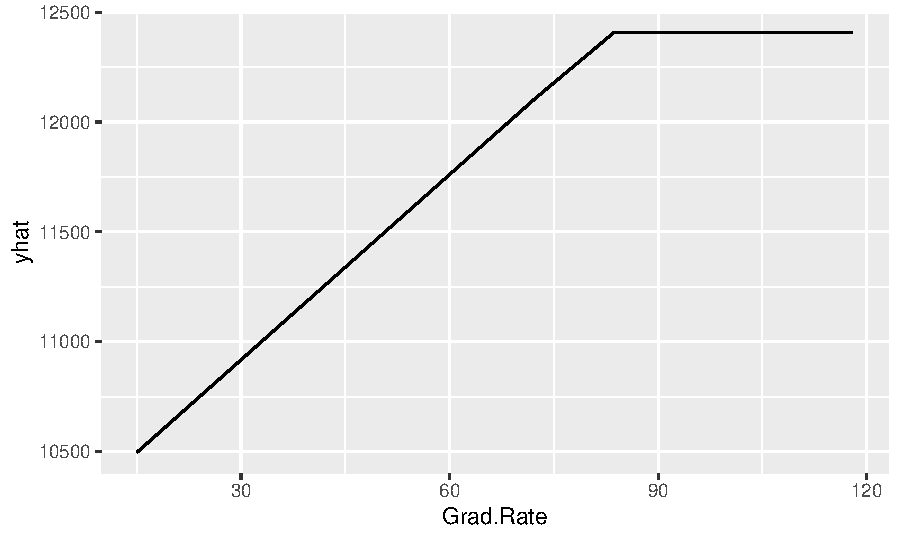
\includegraphics[width=0.9\linewidth]{HW2_co2554_files/figure-latex/MARS-2}

\begin{Shaded}
\begin{Highlighting}[]
\CommentTok{\# test error}
\NormalTok{pred.mars }\OtherTok{\textless{}{-}} \FunctionTok{predict}\NormalTok{(mars.fit, }\AttributeTok{newdata =}\NormalTok{ testing\_data)}

\NormalTok{test.error.mars }\OtherTok{\textless{}{-}} \FunctionTok{mean}\NormalTok{((pred.mars }\SpecialCharTok{{-}}\NormalTok{ y2)}\SpecialCharTok{\^{}}\DecValTok{2}\NormalTok{)}
\end{Highlighting}
\end{Shaded}

The regression function for the MARS model is \textbf{f(Outstate) =
9748.1791 + 0.4632⋅h(Apps−3646) − 1.8972⋅h(2279-Accept) +
6.3690⋅h(913-Enroll) − 1.9849⋅h(Enroll−913) − 1.9452⋅h(1363-F.Undergrad)
− 0.6939⋅h(5895-Room.Board) + 0.8542⋅h(1230-Personal) +
25.4428⋅h(perc.alumni−6) + 0.7506⋅h(Expend−6864) −
0.7703⋅h(Expend−15387) − 28.1240⋅h(83-Grad.Rate)}. The test error is
\ensuremath{3.4360573\times 10^{6}}.

\newpage

\hypertarget{c-construct-a-generalized-additive-model-gam-to-predict-the-response-variable.-does-your-gam-model-include-all-the-predictors-for-the-nonlinear-terms-included-in-your-model-generate-plots-to-visualize-these-relationships-and-discuss-your-observations.-report-the-test-error.}{%
\section{1c) Construct a generalized additive model (GAM) to predict the
response variable. Does your GAM model include all the predictors? For
the nonlinear terms included in your model, generate plots to visualize
these relationships and discuss your observations. Report the test
error.}\label{c-construct-a-generalized-additive-model-gam-to-predict-the-response-variable.-does-your-gam-model-include-all-the-predictors-for-the-nonlinear-terms-included-in-your-model-generate-plots-to-visualize-these-relationships-and-discuss-your-observations.-report-the-test-error.}}

\begin{Shaded}
\begin{Highlighting}[]
\FunctionTok{set.seed}\NormalTok{(}\DecValTok{2}\NormalTok{)}

\CommentTok{\# fit a GAM model using 10{-}fold cross{-}validation}
\NormalTok{gam.fit }\OtherTok{\textless{}{-}} \FunctionTok{train}\NormalTok{(x, y,}
                  \AttributeTok{method =} \StringTok{"gam"}\NormalTok{,}
                  \AttributeTok{tuneGrid =} \FunctionTok{data.frame}\NormalTok{(}\AttributeTok{method =} \StringTok{"GCV.Cp"}\NormalTok{, }\AttributeTok{select =} \FunctionTok{c}\NormalTok{(}\ConstantTok{TRUE}\NormalTok{, }\ConstantTok{FALSE}\NormalTok{)),}
                  \AttributeTok{trControl =}\NormalTok{ ctrl)}
\end{Highlighting}
\end{Shaded}

\begin{verbatim}
## Loading required package: mgcv
\end{verbatim}

\begin{verbatim}
## Loading required package: nlme
\end{verbatim}

\begin{verbatim}
## 
## Attaching package: 'nlme'
\end{verbatim}

\begin{verbatim}
## The following object is masked from 'package:dplyr':
## 
##     collapse
\end{verbatim}

\begin{verbatim}
## This is mgcv 1.9-1. For overview type 'help("mgcv-package")'.
\end{verbatim}

\begin{Shaded}
\begin{Highlighting}[]
\NormalTok{gam.fit}\SpecialCharTok{$}\NormalTok{bestTune}
\end{Highlighting}
\end{Shaded}

\begin{verbatim}
##   select method
## 1  FALSE GCV.Cp
\end{verbatim}

\begin{Shaded}
\begin{Highlighting}[]
\CommentTok{\# for non{-}linear terms, generate plots to visualize relationships}
\NormalTok{gam.fit}\SpecialCharTok{$}\NormalTok{finalModel}
\end{Highlighting}
\end{Shaded}

\begin{verbatim}
## 
## Family: gaussian 
## Link function: identity 
## 
## Formula:
## .outcome ~ s(perc.alumni) + s(Terminal) + s(Books) + s(PhD) + 
##     s(Grad.Rate) + s(Top10perc) + s(Top25perc) + s(S.F.Ratio) + 
##     s(Personal) + s(P.Undergrad) + s(Room.Board) + s(Enroll) + 
##     s(Accept) + s(F.Undergrad) + s(Apps) + s(Expend)
## 
## Estimated degrees of freedom:
## 2.17 1.00 1.00 2.32 4.49 7.59 1.00 
## 3.74 1.00 1.00 2.50 1.00 2.84 6.17 
## 3.89 7.39  total = 50.1 
## 
## GCV score: 2689385
\end{verbatim}

\begin{Shaded}
\begin{Highlighting}[]
\FunctionTok{plot}\NormalTok{(gam.fit}\SpecialCharTok{$}\NormalTok{finalModel)}
\end{Highlighting}
\end{Shaded}

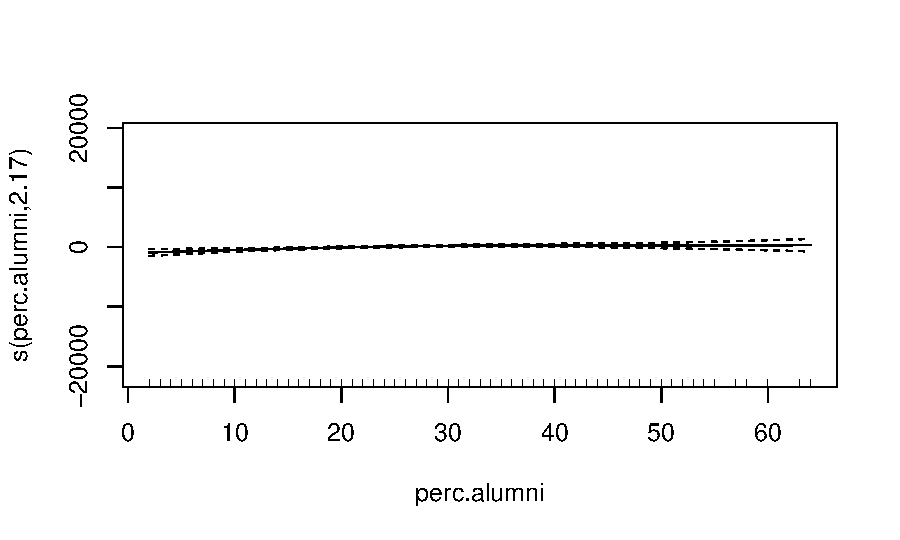
\includegraphics[width=0.9\linewidth]{HW2_co2554_files/figure-latex/GAM-1}
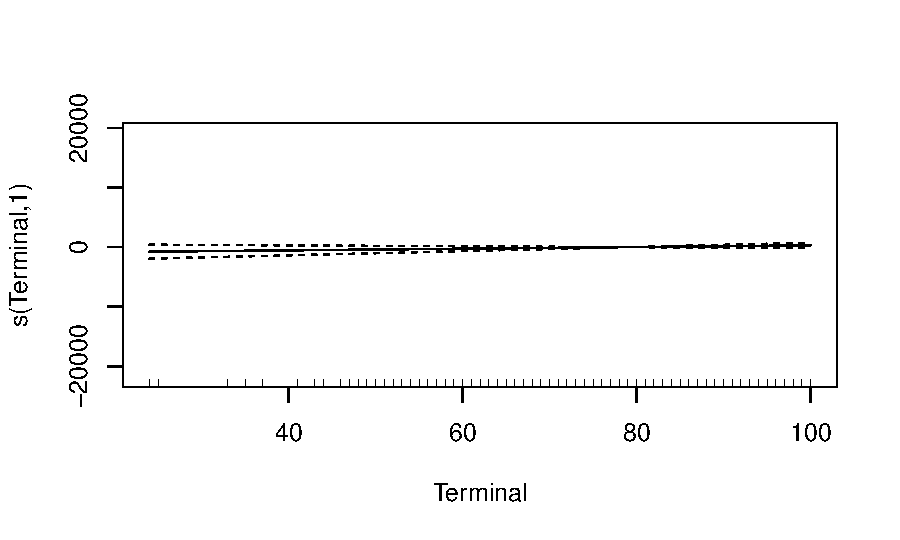
\includegraphics[width=0.9\linewidth]{HW2_co2554_files/figure-latex/GAM-2}
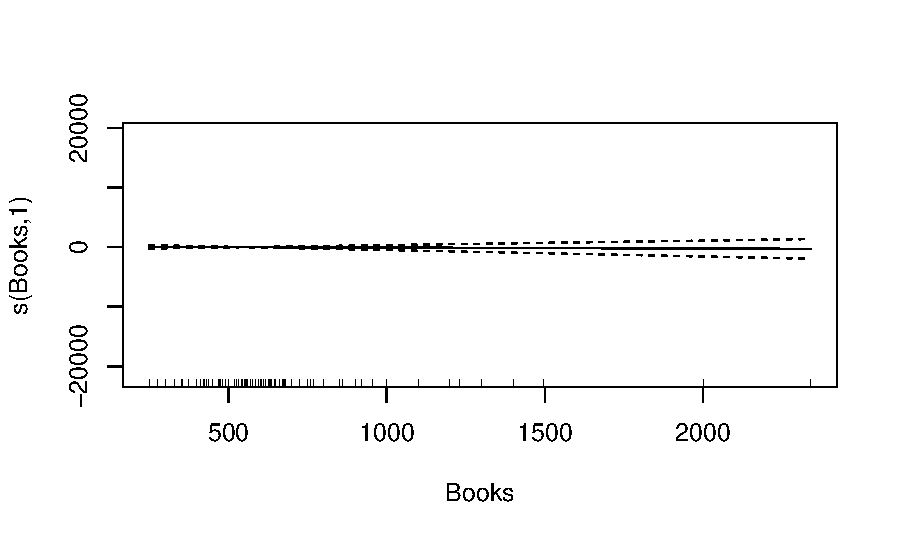
\includegraphics[width=0.9\linewidth]{HW2_co2554_files/figure-latex/GAM-3}
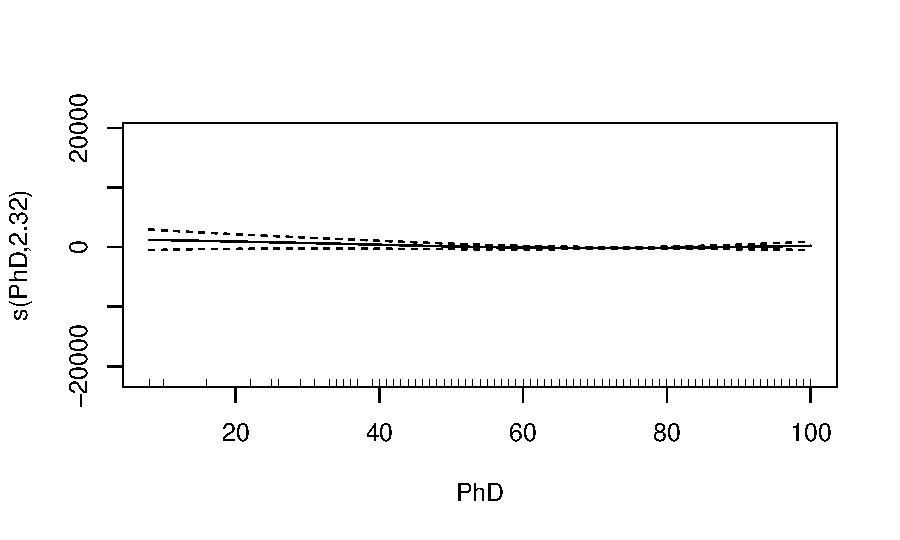
\includegraphics[width=0.9\linewidth]{HW2_co2554_files/figure-latex/GAM-4}
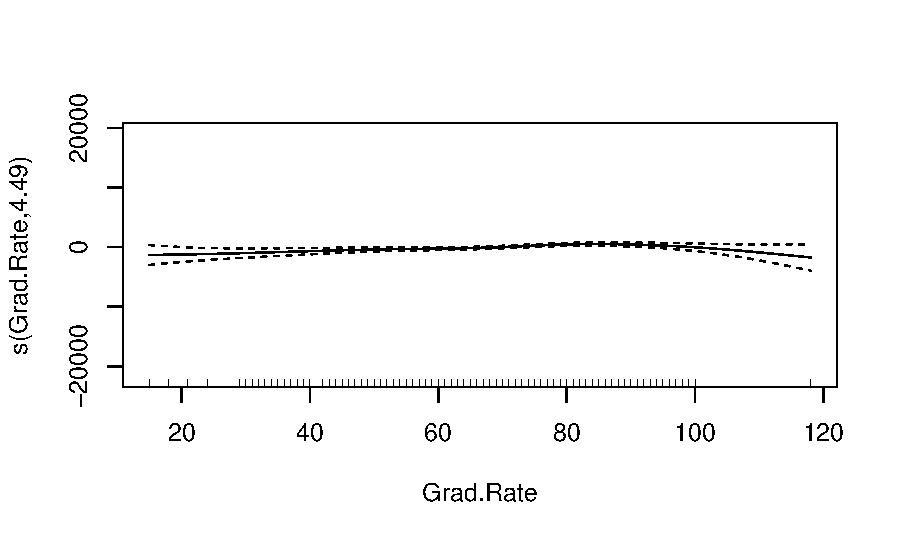
\includegraphics[width=0.9\linewidth]{HW2_co2554_files/figure-latex/GAM-5}
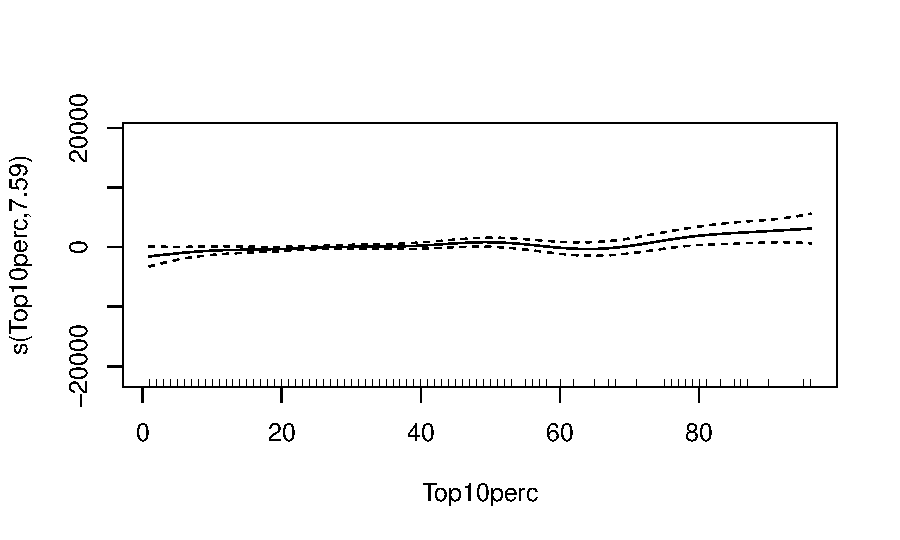
\includegraphics[width=0.9\linewidth]{HW2_co2554_files/figure-latex/GAM-6}
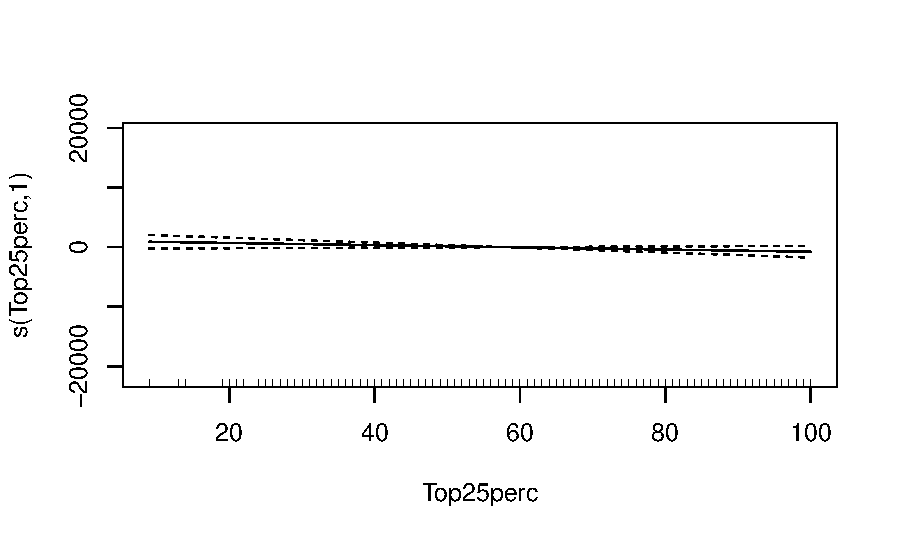
\includegraphics[width=0.9\linewidth]{HW2_co2554_files/figure-latex/GAM-7}
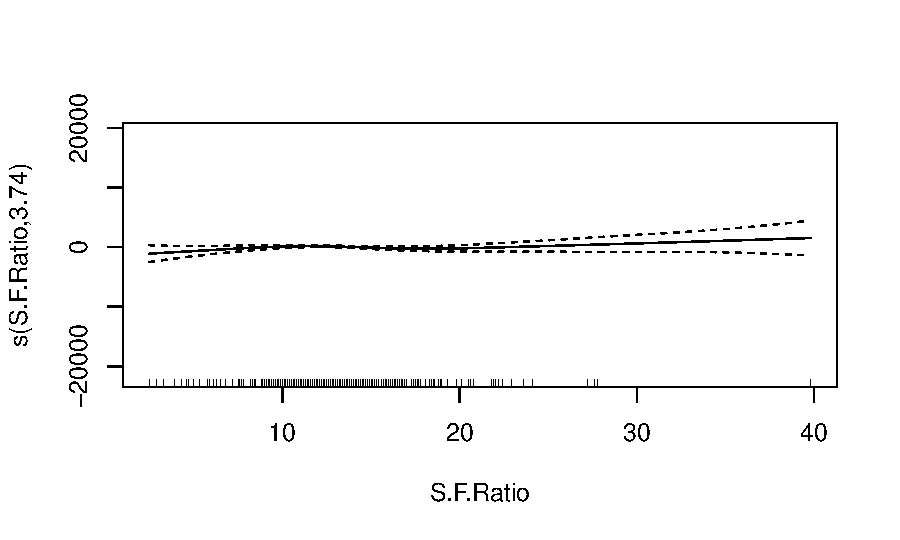
\includegraphics[width=0.9\linewidth]{HW2_co2554_files/figure-latex/GAM-8}
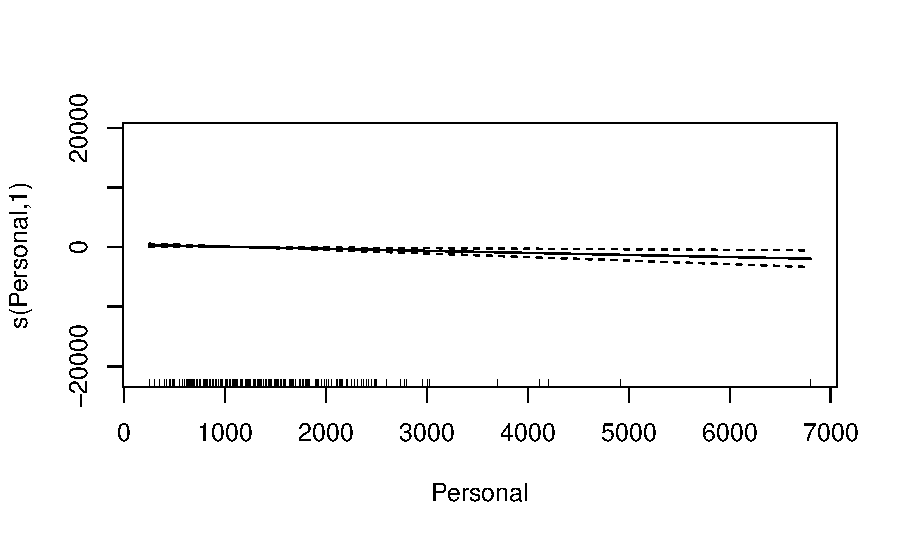
\includegraphics[width=0.9\linewidth]{HW2_co2554_files/figure-latex/GAM-9}
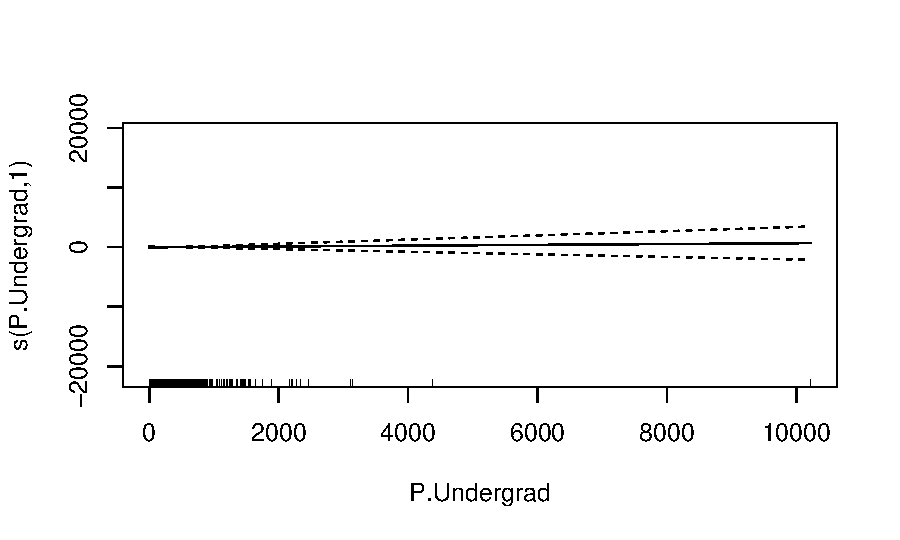
\includegraphics[width=0.9\linewidth]{HW2_co2554_files/figure-latex/GAM-10}
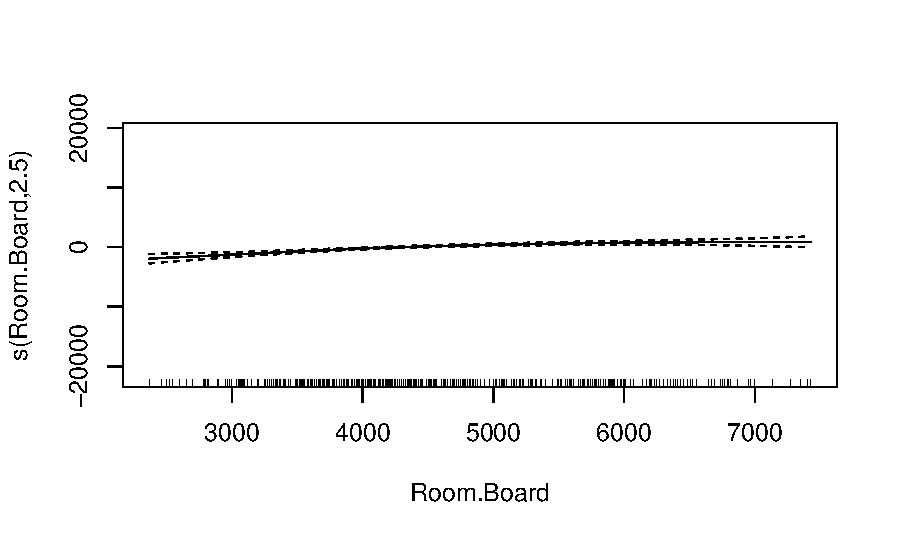
\includegraphics[width=0.9\linewidth]{HW2_co2554_files/figure-latex/GAM-11}
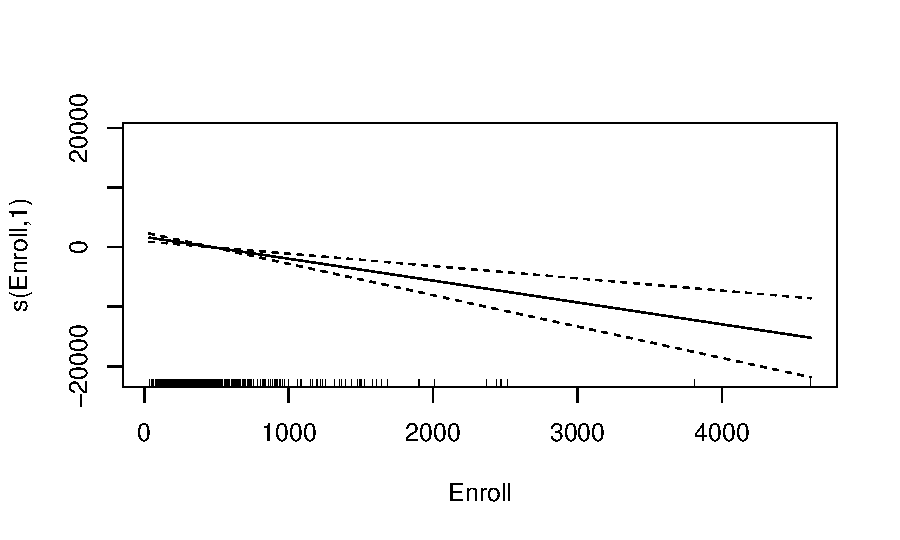
\includegraphics[width=0.9\linewidth]{HW2_co2554_files/figure-latex/GAM-12}
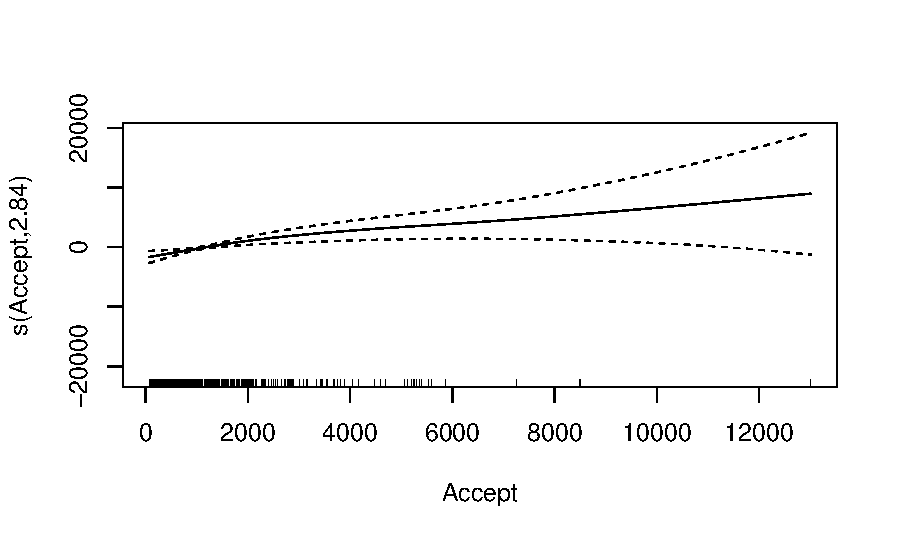
\includegraphics[width=0.9\linewidth]{HW2_co2554_files/figure-latex/GAM-13}
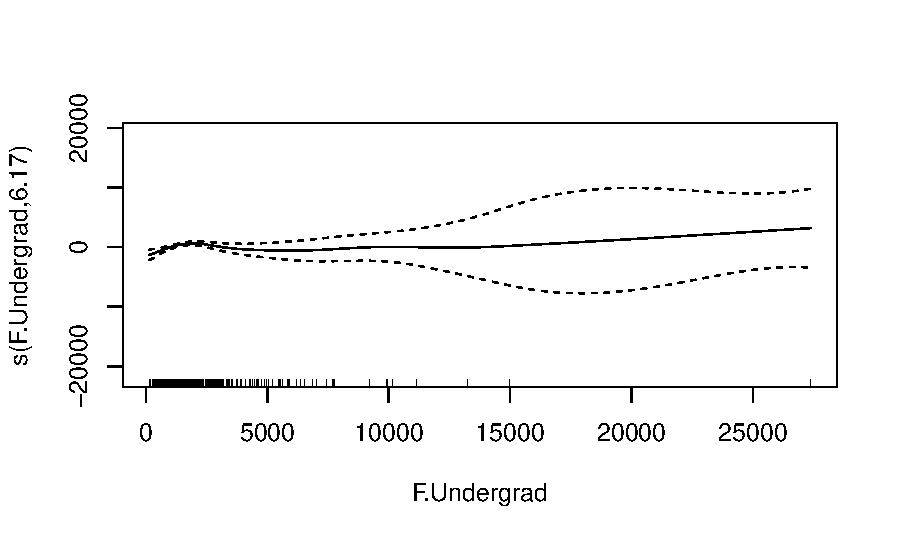
\includegraphics[width=0.9\linewidth]{HW2_co2554_files/figure-latex/GAM-14}
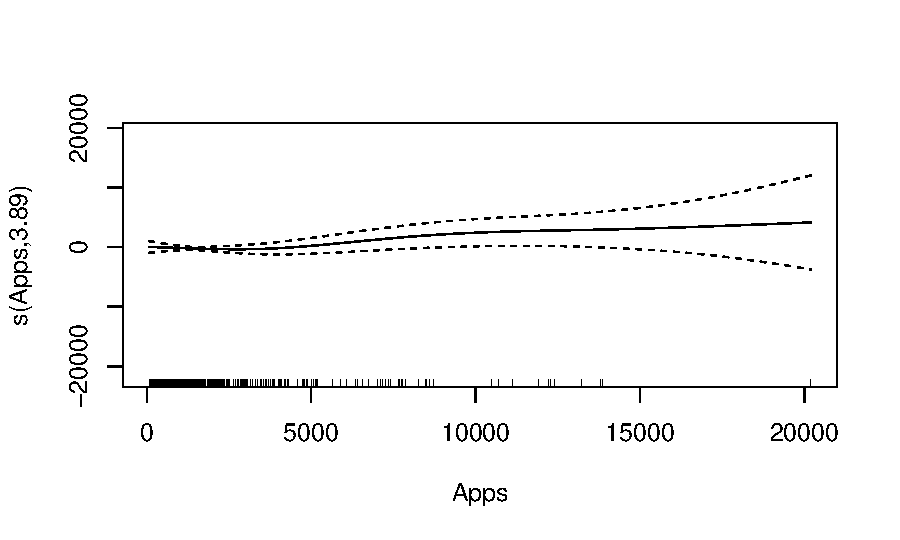
\includegraphics[width=0.9\linewidth]{HW2_co2554_files/figure-latex/GAM-15}
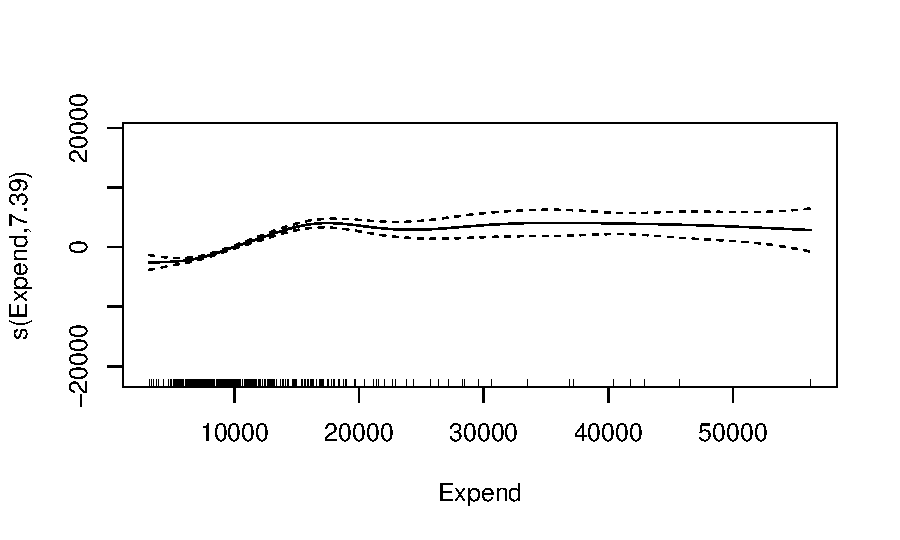
\includegraphics[width=0.9\linewidth]{HW2_co2554_files/figure-latex/GAM-16}

\begin{Shaded}
\begin{Highlighting}[]
\CommentTok{\# report test error}
\NormalTok{pred.gam }\OtherTok{\textless{}{-}} \FunctionTok{predict}\NormalTok{(gam.fit, }\AttributeTok{newdata =}\NormalTok{ testing\_data)}

\NormalTok{test.error.gam }\OtherTok{\textless{}{-}} \FunctionTok{mean}\NormalTok{((pred.gam }\SpecialCharTok{{-}}\NormalTok{ y2)}\SpecialCharTok{\^{}}\DecValTok{2}\NormalTok{)}
\end{Highlighting}
\end{Shaded}

The best fit GAM model does include all predictors. From the final
models plots, we can see that some predictors are more linear than
others. The test error is \ensuremath{3.4345234\times 10^{6}}.

\newpage

\hypertarget{d-in-this-dataset-would-you-favor-a-mars-model-over-a-linear-model-for-predicting-out-of-state-tuition-if-so-why-more-broadly-in-general-applications-do-you-consider-a-mars-model-to-be-superior-to-a-linear-model-please-share-your-reasoning.}{%
\section{1d) In this dataset, would you favor a MARS model over a linear
model for predicting out-of-state tuition? If so, why? More broadly, in
general applications, do you consider a MARS model to be superior to a
linear model? Please share your
reasoning.}\label{d-in-this-dataset-would-you-favor-a-mars-model-over-a-linear-model-for-predicting-out-of-state-tuition-if-so-why-more-broadly-in-general-applications-do-you-consider-a-mars-model-to-be-superior-to-a-linear-model-please-share-your-reasoning.}}

\begin{Shaded}
\begin{Highlighting}[]
\FunctionTok{set.seed}\NormalTok{(}\DecValTok{2}\NormalTok{)}

\CommentTok{\# fit a linear model using 10{-}fold cross{-}validation}
\NormalTok{lm.fit }\OtherTok{\textless{}{-}} \FunctionTok{train}\NormalTok{(x, y, }
                \AttributeTok{method =} \StringTok{"lm"}\NormalTok{,}
                \AttributeTok{trControl =}\NormalTok{ ctrl)}

\FunctionTok{summary}\NormalTok{(lm.fit)}
\end{Highlighting}
\end{Shaded}

\begin{verbatim}
## 
## Call:
## lm(formula = .outcome ~ ., data = dat)
## 
## Residuals:
##    Min     1Q Median     3Q    Max 
##  -6611  -1248     -7   1349   9810 
## 
## Coefficients:
##              Estimate Std. Error t value Pr(>|t|)    
## (Intercept) 752.97152  963.39650   0.782  0.43489    
## Apps         -0.04677    0.11802  -0.396  0.69207    
## Accept        1.33042    0.20335   6.542 1.70e-10 ***
## Enroll       -3.83350    0.91337  -4.197 3.28e-05 ***
## Top10perc    30.21342   15.52858   1.946  0.05234 .  
## Top25perc     0.22821   12.58307   0.018  0.98554    
## F.Undergrad   0.06437    0.14400   0.447  0.65508    
## P.Undergrad  -0.19878    0.16435  -1.210  0.22711    
## Room.Board    0.87381    0.11536   7.575 2.18e-13 ***
## Books         0.36615    0.54397   0.673  0.50123    
## Personal     -0.48636    0.15441  -3.150  0.00175 ** 
## PhD           6.58415   11.93575   0.552  0.58148    
## Terminal     32.39712   13.16108   2.462  0.01422 *  
## S.F.Ratio   -37.67851   31.82476  -1.184  0.23708    
## perc.alumni  39.30520    9.53167   4.124 4.47e-05 ***
## Expend        0.16060    0.02711   5.923 6.42e-09 ***
## Grad.Rate    20.39531    7.25323   2.812  0.00515 ** 
## ---
## Signif. codes:  0 '***' 0.001 '**' 0.01 '*' 0.05 '.' 0.1 ' ' 1
## 
## Residual standard error: 2000 on 435 degrees of freedom
## Multiple R-squared:  0.7358, Adjusted R-squared:  0.7261 
## F-statistic: 75.73 on 16 and 435 DF,  p-value: < 2.2e-16
\end{verbatim}

\begin{Shaded}
\begin{Highlighting}[]
\CommentTok{\# compare models}
\NormalTok{resamp }\OtherTok{\textless{}{-}} \FunctionTok{resamples}\NormalTok{(}\FunctionTok{list}\NormalTok{(}\AttributeTok{lm =}\NormalTok{ lm.fit, }\AttributeTok{mars =}\NormalTok{ mars.fit))}

\FunctionTok{summary}\NormalTok{(resamp)}
\end{Highlighting}
\end{Shaded}

\begin{verbatim}
## 
## Call:
## summary.resamples(object = resamp)
## 
## Models: lm, mars 
## Number of resamples: 10 
## 
## MAE 
##          Min.  1st Qu.   Median     Mean  3rd Qu.     Max. NA's
## lm   1427.528 1578.173 1615.828 1608.826 1674.692 1752.230    0
## mars 1138.836 1239.576 1320.672 1321.704 1425.698 1497.191    0
## 
## RMSE 
##          Min.  1st Qu.   Median     Mean  3rd Qu.     Max. NA's
## lm   1770.494 1950.509 2030.364 2047.597 2114.502 2393.058    0
## mars 1377.340 1548.527 1712.939 1688.556 1831.993 1956.649    0
## 
## Rsquared 
##           Min.   1st Qu.    Median      Mean   3rd Qu.      Max. NA's
## lm   0.6577688 0.7142791 0.7249317 0.7204843 0.7408093 0.7704528    0
## mars 0.7384265 0.7672405 0.8068437 0.8053855 0.8427477 0.8636907    0
\end{verbatim}

\begin{Shaded}
\begin{Highlighting}[]
\FunctionTok{parallelplot}\NormalTok{(resamp, }\AttributeTok{metric =} \StringTok{"RMSE"}\NormalTok{)}
\end{Highlighting}
\end{Shaded}

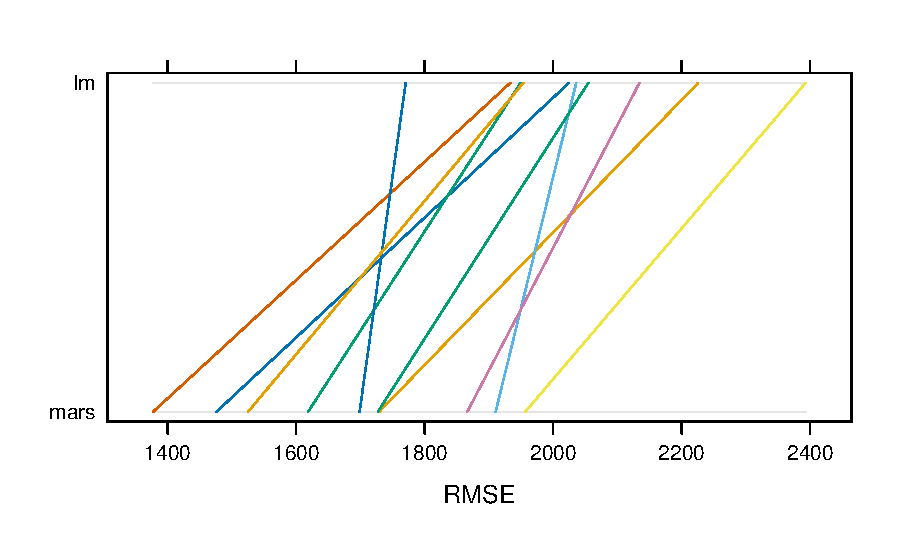
\includegraphics[width=0.9\linewidth]{HW2_co2554_files/figure-latex/model_compare-1}

\begin{Shaded}
\begin{Highlighting}[]
\FunctionTok{bwplot}\NormalTok{(resamp, }\AttributeTok{metric =} \StringTok{"RMSE"}\NormalTok{)}
\end{Highlighting}
\end{Shaded}

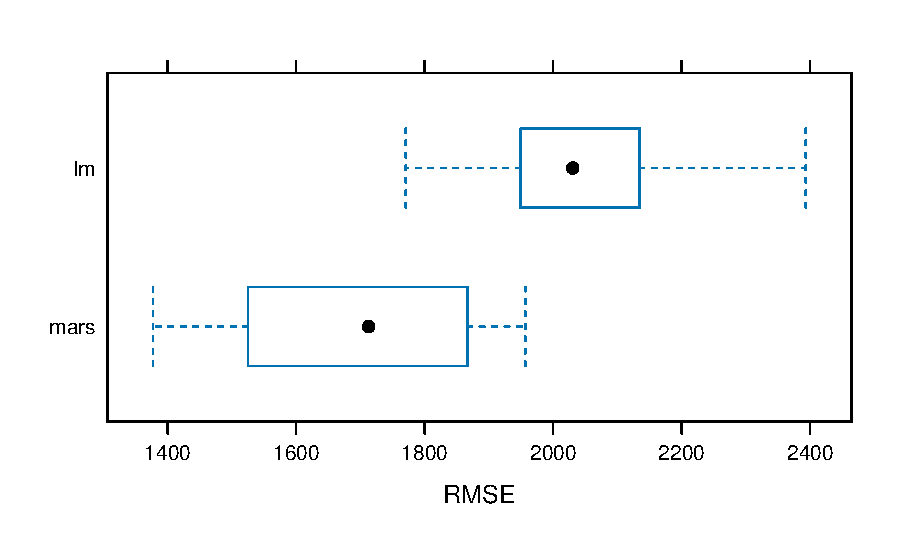
\includegraphics[width=0.9\linewidth]{HW2_co2554_files/figure-latex/model_compare-2}
From the resampling summary, I believe the best model is the MARS since
it has the smallest mean and median RMSE value. I would prefer fitting a
MARS model over a linear model mostly because of its flexibility. MARS
models can capture non-linear relationships, can capture interactions
between variables, and are generally more robust.

\end{document}
